\section{Optimal Control of Pitch and Travel with Feedback (LQ)}\label{sec:prob3}
In this section we introduce feedback to correct for deviations from the optimal trajectory caused by modelling errors. We use a linear-quadratic regulator, and compute the optimal feedback gain by solving a discrete algebraic Riccati-equation. We also discuss if MPC could be a good alternative to LQR.

\subsection{Implementing feedback}
Feedback for the system is introduced by adding a correcting term to the optimal input, before passing it into the internal regulators,
\begin{equation}
    u_k = u_k^* - K^T(x_k - x_k^*)
\end{equation}
Here $x^*$ is the optimal trajectory and $u^*$ is the optimal input sequence. The block diagram structure of the helicopter with feedback can be seen in figure \ref{fig:simulink_day3}. $K$ is selected as the optimal feedback gain, found by minimizing the objective function
\begin{equation}
    \label{eq:cost_function_lqr_day3}
    J = \sum_{i=0}^\infty {\Delta x_{i+1}^TQ\Delta x_{i+1} + \Delta u_{i}^TR\Delta u_{i}}
\end{equation}
subject to the linear model $\Delta x_{i+1} = A\Delta x + B\Delta u$, where $\Delta x$ and $\Delta u$ are deviations from the optimal trajectory. Q and R are weighting matrices that can be chosen to penalize individual deviations in states or input. We discuss how we tuned these matrices in the next section.

\subsection{Results}
We used the built-in MATLAB function dlqr to solve the Riccati-equation for the optimization problem corresponding to (\ref{eq:cost_function_lqr_day3}), and compute the optimal gain $K$. We chose $Q$ and $R$ to be diagonal matrices, with $R$ constant and equal to the identity. $Q$ was then tuned by increasing or decreasing the weights along the diagonal.

\begin{figure}[htb]
    \centering
        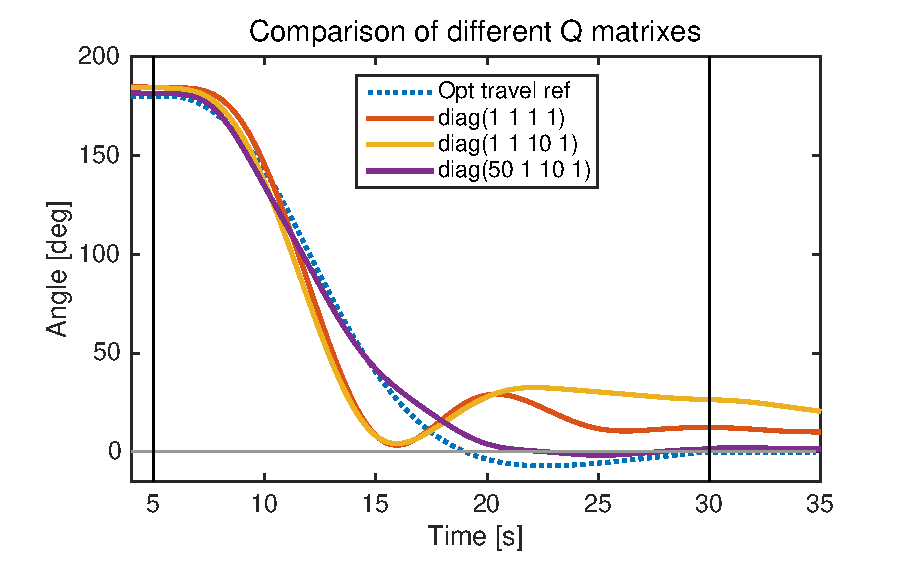
\includegraphics[width=1.0\textwidth]{figures/day3/plot_day3_allQ}
        % \makebox[\textwidth][c]{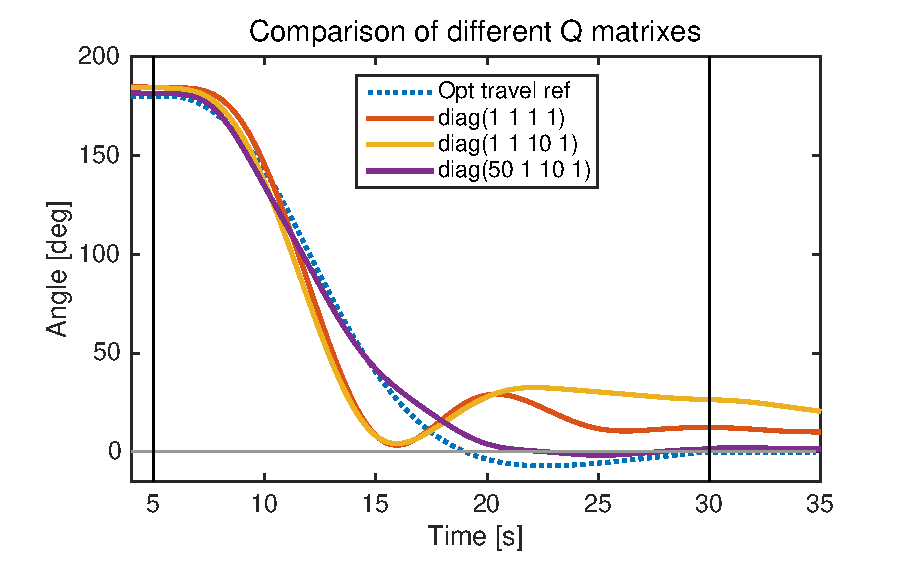
\includegraphics[width=1.1\textwidth]{figures/day3/plot_day3_allQ}}
    \caption{Measured travel trajectory for different values of Q}
    \label{fig:day3_plot_allQ}
\end{figure}

Figure \ref{fig:day3_plot_allQ} shows the measured travel trajectory with different values of $Q$, compared to the computed optimal path. We found that by weighting travel more than pitch (50 1 1 1), the helicopter followed the travel trajectory closer than when weighting all states the same. Weighting deviation in pitch more than travel (1 1 10 1) gave a bad result. The reason for this was that the optimal pitch setpoint was computed for an unrealistic model.

\subsection{Comparison between LQR and MPC}
The way to implement an MPC controller would be to calculate a new optimal trajectory at each time step. The first time step of each calculated optimal input sequence should then be used as the input $u_t$ for that time step.

The advantages of using MPC instead of LQR is that it gives the possibility to have constraints in the regulator. MPC might also result in a trajectory demanding less input, and provides implicit feedback. As we have already observed, feedback is a necessity for the control of a system with modelling errors and disturbances.
The main disadvantage of using MPC is that the heavy calculations of finding an optimal trajectory would have to be processed during run time, hence it might not be able to control a system as fast as a helicopter.
The control hierarchy with MPC would have replaced the Advanced control layer by the Optimization layer, leading to one less layer in the hierarchy.
